% ------------------------------------------------------------------------------
% TYPO3 CMS 8 LTS - What's New - Chapter "In-Depth Changes" (English Version)
%
% @author	Michael Schams <schams.net>
% @license	Creative Commons BY-NC-SA 3.0
% @link		http://typo3.org/download/release-notes/whats-new/
% @language	English
% ------------------------------------------------------------------------------
% LTXE-CHAPTER-UID:		5ebcecbe-66abfa57-cf38bc00-aa637965
% LTXE-CHAPTER-NAME:	In-Depth Changes
% ------------------------------------------------------------------------------

\section{In-Depth Changes}
\begin{frame}[fragile]
	\frametitle{In-Depth Changes}

	\begin{center}\huge{\color{typo3darkgrey}\textbf{In-Depth Changes}}\end{center}
	\begin{center}\large{\textit{Awesome new features and improvements under the hood}}\end{center}

\end{frame}

% ------------------------------------------------------------------------------
% LTXE-SLIDE-START
% LTXE-SLIDE-UID:		b9b259e4-9d35ace7-edff1014-7390d1d1
% LTXE-SLIDE-TITLE:		#69794: Support PECL-memcached in MemcachedBackend
% ------------------------------------------------------------------------------
\begin{frame}[fragile]
	\frametitle{In-Depth Changes}
	\framesubtitle{Support PECL-memcached in MemcachedBackend}

	% decrease font size for code listing
	\lstset{basicstyle=\tiny\ttfamily}

	\begin{itemize}

		\item Support for the PECL module "memcached" has been added to the
			MemcachedBackend of the Caching Framework

		\item If both, "memcache" and "memcached" are installed, "memcache"
			is used to avoid being a breaking change.

		\item An integrator may set the option \texttt{peclModule} to use the
			preferred PECL module:

			\begin{lstlisting}
				$GLOBALS['TYPO3_CONF_VARS']['SYS']['caching']['cacheConfigurations']['my_memcached'] = [
				  'frontend' => \TYPO3\CMS\Core\Cache\Frontend\VariableFrontend::class
				  'backend' => \TYPO3\CMS\Core\Cache\Backend\MemcachedBackend::class,
				  'options' => [
				    'peclModule' => 'memcached',
				    'servers' => [
				      'localhost',
				      'server2:port'
				    ]
				  ]
				];
			\end{lstlisting}

	\end{itemize}

\end{frame}


% ------------------------------------------------------------------------------
% LTXE-SLIDE-START
% LTXE-SLIDE-UID:		ef8c124e-f902453a-d48770b9-4cf86545
% LTXE-SLIDE-TITLE:		#73042: Native support for Symfony Console (1)
% ------------------------------------------------------------------------------
\begin{frame}[fragile]
	\frametitle{In-Depth Changes}
	\framesubtitle{Native support for Symfony Console (1)}

	% decrease font size for code listing
	\lstset{basicstyle=\tiny\ttfamily}

	\begin{itemize}

		\item TYPO3 supports the Symfony Console component out-of-the-box now by providing
			a new command line script located in \texttt{typo3/sysext/core/bin/typo3}.
			On TYPO3 instances installed via Composer, the binary is linked into the
			\texttt{bin}-directory, e.g. \texttt{bin/typo3}.

		\item The new binary still supports the existing command line arguments when no
			proper Symfony Console command was found as a fallback.

		\item Registering a command to be available via the \texttt{typo3} command line
			tool works by putting a \texttt{Configuration/Commands.php} file into any
			installed extension. The content of this file is an associative array, which
			contains the Symfony/Console/Command classes. The key is the name of the
			command to be called as the first argument to \texttt{typo3}.
	\end{itemize}

\end{frame}

% ------------------------------------------------------------------------------
% LTXE-SLIDE-START
% LTXE-SLIDE-UID:		28b018bb-21804fa1-c578f0ff-fc16cbb1
% LTXE-SLIDE-TITLE:		#73042: Native support for Symfony Console (2)
% ------------------------------------------------------------------------------
\begin{frame}[fragile]
	\frametitle{In-Depth Changes}
	\framesubtitle{Native support for Symfony Console (2)}

	% decrease font size for code listing
	\lstset{basicstyle=\tiny\ttfamily}

	\begin{itemize}

		\item A required parameter when registering a command is the \texttt{class} property.
			Optionally the \texttt{user} parameter can be set so a backend user is logged
			in when calling the command.

		\item Typical example of a \texttt{Configuration/Commands.php} file:

			\begin{lstlisting}
				return [
				  'backend:lock' => [
				    'class' => \TYPO3\CMS\Backend\Command\LockBackendCommand::class
				  ],
				  'referenceindex:update' => [
				    'class' => \TYPO3\CMS\Backend\Command\ReferenceIndexUpdateCommand::class,
				    'user' => '_cli_lowlevel'
				  ]
				];
			\end{lstlisting}

	\end{itemize}

\end{frame}

% ------------------------------------------------------------------------------
% LTXE-SLIDE-START
% LTXE-SLIDE-UID:		fc16cbb1-21804fa1-c578f0ff-28b018bb
% LTXE-SLIDE-TITLE:		#73042: Native support for Symfony Console (3)
% ------------------------------------------------------------------------------
\begin{frame}[fragile]
	\frametitle{In-Depth Changes}
	\framesubtitle{Native support for Symfony Console (3)}

	% decrease font size for code listing
	\lstset{basicstyle=\tiny\ttfamily}

	\begin{itemize}

		\item An example call could look like:
			\begin{lstlisting}
				bin/typo3 backend:lock http://example.com/maintenance.html
			\end{lstlisting}

		\item For a non-Composer installation:
			\begin{lstlisting}
				typo3/sysext/core/bin/typo3 backend:lock http://example.com/maintenance.html
			\end{lstlisting}

	\end{itemize}

\end{frame}


% ------------------------------------------------------------------------------
% LTXE-SLIDE-START
% LTXE-SLIDE-UID:		dd31e5d5-ca09ae5e-eb87d926-0ffe8f0a
% LTXE-SLIDE-TITLE:		Low-level parameters changes (1)
% ------------------------------------------------------------------------------
\begin{frame}[fragile]
	\frametitle{In-Depth Changes}
	\framesubtitle{Low-level Parameter Changes (1)}

	% changes: #78417, #78439, #78520, #78552, #78577, #78623, #78627 and #78895

	\begin{itemize}
		\item Low-level commands listed below use the Symfony Console now
		\item New commands behave like the old ones, but allow using certain parameters

			\begin{itemize}
				\item \texttt{DeletedRecordsCommand}
				\item \texttt{CleanFlexFormsRecordsCommand}
				\item \texttt{OrphanRecordsCommand}
				\item \texttt{LostFilesCommand}
				\item \texttt{MissingFilesCommand}
				\item \texttt{MissingRelationsCommand}
				\item \texttt{DoubleFilesCommand}
				\item \texttt{RteImagesCommand}
			\end{itemize}

	\end{itemize}

\end{frame}

% ------------------------------------------------------------------------------
% LTXE-SLIDE-START
% LTXE-SLIDE-UID:		3a9d25bb-d948368d-e2a92666-6170eaad
% LTXE-SLIDE-TITLE:		Low-level parameters changes (2)
% ------------------------------------------------------------------------------
\begin{frame}[fragile]
	\frametitle{In-Depth Changes}
	\framesubtitle{Low-level Parameter Changes (2)}

	% changes: #78417, #78439, #78520, #78552, #78577, #78623, #78627 and #78895

	\begin{itemize}
		\item Related PHP classes have been removed\newline
			\smaller(e.g. \texttt{TYPO3\textbackslash
				CMS\textbackslash
				Lowlevel\textbackslash
				DeletedRecordsCommand})
			\normalsize

		\item Executing the command via \texttt{cli\_dispatch} does not work anymore\newline
			\smaller(e.g. \texttt{typo3/cli\_dispatch lowlevel cleaner deleted})\normalsize
		\item Calling the PHP class results in a fatal PHP error now

		\item Commands can now be executed via CLI as follows:\newline
			\smaller\texttt{/typo3/sysext/core/bin/typo3 cleanup:<command>}\normalsize\newline
			for example:\newline
			\smaller\texttt{/typo3/sysext/core/bin/typo3 cleanup:deletedrecords}\normalsize

	\end{itemize}

\end{frame}

% ------------------------------------------------------------------------------
% LTXE-SLIDE-START
% LTXE-SLIDE-UID:		1626edc6-8d93ff84-f64178bf-8e7650df
% LTXE-SLIDE-TITLE:		#73050: Cryptographically secure pseudorandom number generator
% ------------------------------------------------------------------------------
\begin{frame}[fragile]
	\frametitle{In-Depth Changes}
	\framesubtitle{Cryptographically secure pseudorandom number generator}

	% decrease font size for code listing
	\lstset{basicstyle=\tiny\ttfamily}

	\begin{itemize}

		\item A new cryptographically secure pseudo-random number generator (CSPRNG) has been
			implemented in the TYPO3 core.\newline
			It takes advantage of the new CSPRNG functions in PHP 7.

		\item The API resides in the class
			\texttt{\textbackslash
				TYPO3\textbackslash
				CMS\textbackslash
				Core\textbackslash
				Crypto\textbackslash
				Random}

		\item Example:

			\begin{lstlisting}
				use \TYPO3\CMS\Core\Crypto\Random;
				use \TYPO3\CMS\Core\Utility\GeneralUtility;

				// Retrieving random bytes
				$someRandomString = GeneralUtility::makeInstance(Random::class)->generateRandomBytes(64);

				// Rolling the dice..
				$tossedValue = GeneralUtility::makeInstance(Random::class)->generateRandomInteger(1, 6);
			\end{lstlisting}

	\end{itemize}

\end{frame}

% ------------------------------------------------------------------------------
% LTXE-SLIDE-START
% LTXE-SLIDE-UID:		2c656d9e-38b9be7a-d590cb6e-21eccd4d
% LTXE-SLIDE-TITLE:		#28230: Password hashing algorithm: PBKDF2
% ------------------------------------------------------------------------------
\begin{frame}[fragile]
	\frametitle{In-Depth Changes}
	\framesubtitle{Password hashing algorithm: PBKDF2}

	\begin{itemize}

		\item A new password hashing algorithm "PBKDF2" has been added to the system extension "saltedpasswords"

		\item PBKDF2 stands for: Password-Based Key Derivation Function 2

		\item The algorithm is designed to be computationally expensive to resist brute force password cracking

	\end{itemize}

\end{frame}

% ------------------------------------------------------------------------------
% LTXE-SLIDE-START
% LTXE-SLIDE-UID:		630de169-c2699a8a-ee44dde5-cf39c2ca
% LTXE-SLIDE-TITLE:		#70056 - PHP Library "Guzzle" (1)
% ------------------------------------------------------------------------------
\begin{frame}[fragile]
	\frametitle{In-Depth Changes}
	\framesubtitle{PHP Library "Guzzle" (1)}

	\begin{itemize}

		\item The PHP library
			"\href{http://docs.guzzlephp.org}{Guzzle}"
			has been added via composer dependency to work as a feature rich
			solution for creating HTTP requests based on the PSR-7 interfaces
			already used within TYPO3

		\item Guzzle auto-detects available underlying adapters available on
			the system, like cURL or stream wrappers and chooses the best
			solution for the system

		\item A TYPO3-specific PHP class called
			\texttt{TYPO3\textbackslash
				CMS\textbackslash
				Core\textbackslash
				Http\textbackslash
				RequestFactory}\newline
			has been added as a simplified wrapper to access Guzzle clients

	\end{itemize}

\end{frame}


% ------------------------------------------------------------------------------
% LTXE-SLIDE-START
% LTXE-SLIDE-UID:		db2b31c1-47321ffe-3ed51ebc-5dd524a4
% LTXE-SLIDE-TITLE:		#70056 - PHP Library "Guzzle" (2)
% ------------------------------------------------------------------------------
\begin{frame}[fragile]
	\frametitle{In-Depth Changes}
	\framesubtitle{PHP Library "Guzzle" (2)}

	% decrease font size for code listing
	\lstset{basicstyle=\tiny\ttfamily}

	\begin{itemize}

		\item The \texttt{RequestFactory} class can be used like this:

			\begin{lstlisting}
				// Initiate RequestFactory

				/** @var \TYPO3\CMS\Core\Http\RequestFactory $requestFactory */
				$requestFactory = GeneralUtility::makeInstance(
				  \TYPO3\CMS\Core\Http\RequestFactory\RequestFactory::class);

				$uri = $additionalOptions = [
				  // additional headers for this specific request
				  'headers' => ['Cache-Control' => 'no-cache'],
				  'allow_redirects' => false,
				  'cookies' => true
				];

				// return a PSR-7 compliant response object
				$response = $requestFactory->request($url, 'GET', $additionalOptions);

				// get the content as a string on a successful request
				if ($response->getStatusCode() === 200) {
				  if ($response->getHeader('Content-Type') === 'text/html') {
				    $content = $response->getBody()->getContents();
				  }
				}
			\end{lstlisting}

	\end{itemize}

\end{frame}

% ------------------------------------------------------------------------------
% LTXE-SLIDE-START
% LTXE-SLIDE-UID:		bd33b29d-c20d1765-f923f78e-43bfb0bf
% LTXE-SLIDE-TITLE:		#74365: Add Linkservice for Unified Referencing Syntax (1)
% ------------------------------------------------------------------------------
\begin{frame}[fragile]
	\frametitle{In-Depth Changes}
	\framesubtitle{Add Linkservice for Unified Referencing Syntax (1)}

	\begin{itemize}

		\item Resources within TYPO3 have been referenced using multiple, different forms of syntax in the past.

		\item TYPO3 now supports a modern and future-proof way of referencing resources using an extensible and
			expressive syntax which is easy to understand.

		\item The next slides explain the syntax using the following simple page link:

			\begin{lstlisting}
				t3://page?uid=13&campaignCode=ABC123
			\end{lstlisting}

	\end{itemize}

\end{frame}

% ------------------------------------------------------------------------------
% LTXE-SLIDE-START
% LTXE-SLIDE-UID:		95f9a663-ea2155a1-5635728b-77a8995c
% LTXE-SLIDE-TITLE:		#74365: Add Linkservice for Unified Referencing Syntax (2)
% ------------------------------------------------------------------------------
\begin{frame}[fragile]
	\frametitle{In-Depth Changes}
	\framesubtitle{Add Linkservice for Unified Referencing Syntax (2)}

	\begin{itemize}

		\item The syntax consists of three parts:

			\begin{itemize}

				\item Namespace (\texttt{t3://})\newline
		   			The namespace is fixed to \texttt{t3://} to ensure the "LinkService" is executed to parse the URN.
					\newline
				\item Resource handler key (\texttt{page})\newline
   					The resource handler key identifies the resource in the TYPO3 available handlers list.
					At the time of writing the following handlers exist: \texttt{page}, \texttt{file} and \texttt{folder}.\newline
					More keys can be configured in an associative array, where the key is the handler key and the value
					is a class implementing the LinkHandlerInterface:\newline
					\texttt{\$TYPO3\_CONF\_VARS['SYS']['linkHandler']}

			\end{itemize}

	\end{itemize}

\end{frame}

% ------------------------------------------------------------------------------
% LTXE-SLIDE-START
% LTXE-SLIDE-UID:		77a8995c-ea2155a1-95f9a663-5635728b
% LTXE-SLIDE-TITLE:		#74365: Add Linkservice for Unified Referencing Syntax (3)
% ------------------------------------------------------------------------------
\begin{frame}[fragile]
	\frametitle{In-Depth Changes}
	\framesubtitle{Add Linkservice for Unified Referencing Syntax (3)}

	\begin{itemize}

		\item ...and the 3rd part:

			\begin{itemize}

				\item Resource parameters (\texttt{?uid=13\&campaignCode=ABC123})\newline
					These are the specific identification parameters that are used by any handler.
					Note that these may carry additional parameters in order to configure the behavior of any handler.

			\end{itemize}

	\end{itemize}

\end{frame}

% ------------------------------------------------------------------------------
% LTXE-SLIDE-START
% LTXE-SLIDE-UID:		af8e73a4-2b315873-bb6e55e4-c0cd82b5
% LTXE-SLIDE-TITLE:		#76008 and #76458: DebuggerUtility::var_dump (1)
% ------------------------------------------------------------------------------
\begin{frame}[fragile]
	\frametitle{In-Depth Changes}
	\framesubtitle{\texttt{DebuggerUtility::var\_dump} (1)}

	\begin{itemize}

		\item The property visibility information has been added to \texttt{DebuggerUtility::var\_dump()}
			\newline
			for each object property in the dump

		\item If a closure is part of the debugging object, the source code of the closure is rendered, too

	\end{itemize}

	\tabto{0.75cm}\textit{See example on the next slide}

\end{frame}

% ------------------------------------------------------------------------------
% LTXE-SLIDE-START
% LTXE-SLIDE-UID:		bb6e55e4-2b315873-c0cd82b5-af8e73a4
% LTXE-SLIDE-TITLE:		#76008 and #76458: DebuggerUtility::var_dump (2)
% ------------------------------------------------------------------------------
\begin{frame}[fragile]
	\frametitle{In-Depth Changes}
	\framesubtitle{\texttt{DebuggerUtility::var\_dump} (2)}

	\begin{figure}
		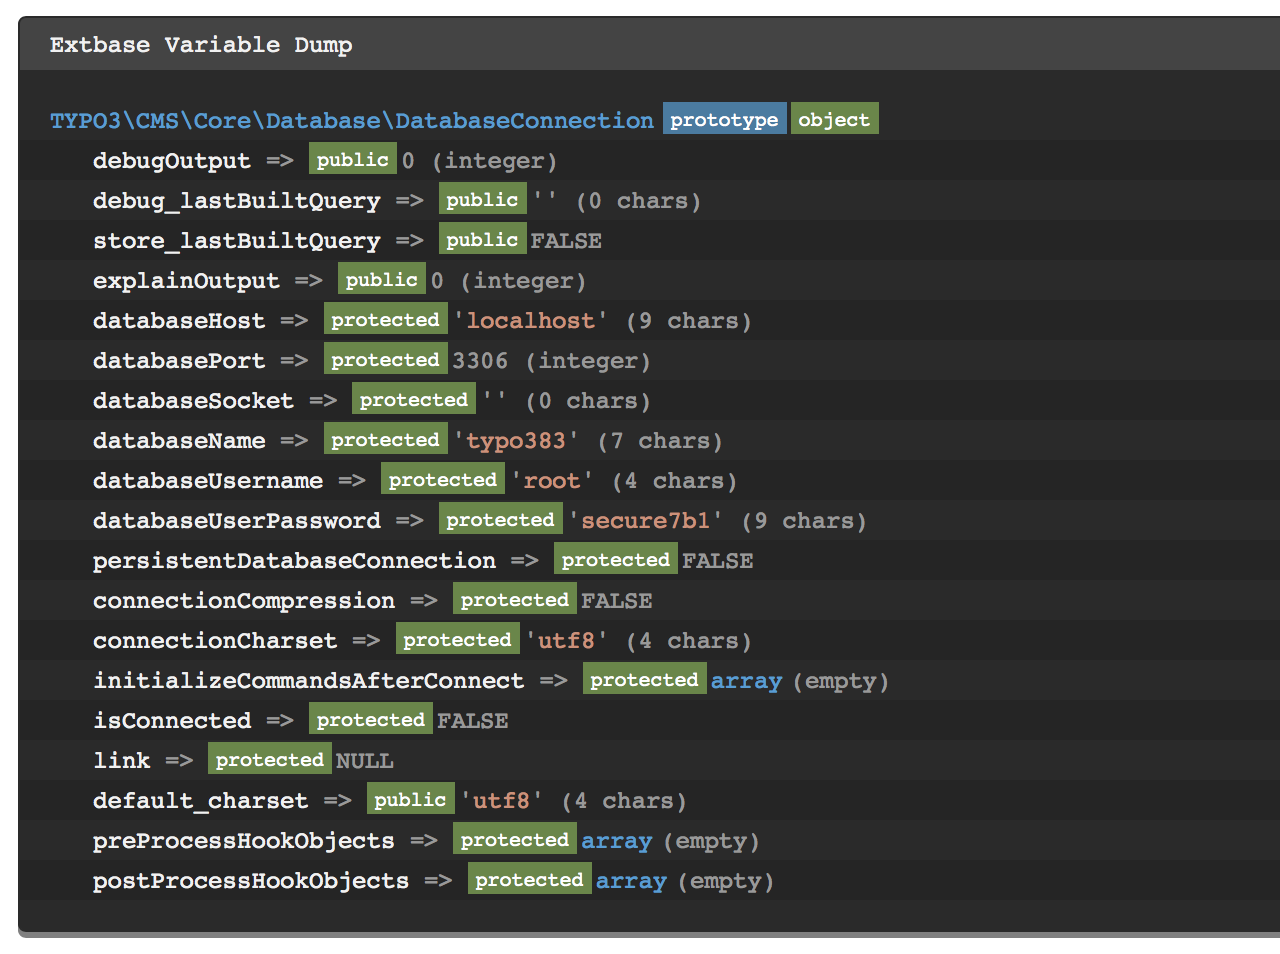
\includegraphics[width=0.65\linewidth]{InDepthChanges/76008.png}
	\end{figure}

\end{frame}

% ------------------------------------------------------------------------------
% LTXE-SLIDE-START
% LTXE-SLIDE-UID:		60a2d39f-f04b8bf1-dc758912-607ed07e
% LTXE-SLIDE-TITLE:		#52286: System Status Updates Report via email
% ------------------------------------------------------------------------------
\begin{frame}[fragile]
	\frametitle{In-Depth Changes}
	\framesubtitle{System Status Updates (Reports)}

	\begin{itemize}
		\item Results of test in the "System Status Updates (reports)" can be sent via email
		\item A checkbox has been added to the job configuration to:

			\begin{itemize}
				\item send an email if the system has warnings or errors
				\item always generate an email
			\end{itemize}

		\item The default is to include warnings and errors only

	\end{itemize}

\end{frame}

% ------------------------------------------------------------------------------
% LTXE-SLIDE-START
% LTXE-SLIDE-UID:		e4e2ead3-c07beb21-e8100580-d0e7c756
% LTXE-SLIDE-TITLE:		#58637: Purge language packs in language module
% ------------------------------------------------------------------------------

%\begin{frame}[fragile]
%	\frametitle{In-Depth Changes}
%	\framesubtitle{Language Packs}
%
%	\begin{itemize}
%		\item Deactivating languages in the module "Languages" left language data remaining
%			in directory \texttt{typo3conf/l10n/<locale>/}
%		\item A "remove"-button has been added, which disables the language and purges the
%			data in the directory
%	\end{itemize}
%
%\end{frame}

% ------------------------------------------------------------------------------
% LTXE-SLIDE-START
% LTXE-SLIDE-UID:		73d888ce-a14c0f6a-d4dec5fb-f7368bb6
% LTXE-SLIDE-TITLE:		#76108, #77349 and #77481 Miscellaneous (1)
% ------------------------------------------------------------------------------
\begin{frame}[fragile]
	\frametitle{In-Depth Changes}
	\framesubtitle{Miscellaneous (1)}

	\begin{itemize}

		\item SVGs and D3 rendering

			\begin{itemize}
				\item As part of the ExtJS removal from the TYPO3 core, the tree within the form editing has been re-worked
				\item Rendering is based on SVGs and D3 now, which comes with a significant performance boost
				\item Re-working the page tree the same way is planned for the near future
			\end{itemize}

		\item Extension icons can be stored in the following directory now:\newline
			\small
				\texttt{Resources/Public/Icons/<filename>}
				(where <filename> can be: \texttt{Extension.png}, \texttt{Extension.svg} or \texttt{Extension.gif})
			\normalsize

		\item The new option \texttt{backendFavicon} in the Extension Manager configuration makes it possible to
			change the favicon of the backend.

	\end{itemize}

\end{frame}

% ------------------------------------------------------------------------------
% LTXE-SLIDE-START
% LTXE-SLIDE-UID:		0907e5d3-a12751cb-23f49488-7a05a208
% LTXE-SLIDE-TITLE:		#78103, #78575 and #75232: Miscellaneous (2)
% ------------------------------------------------------------------------------
\begin{frame}[fragile]
	\frametitle{In-Depth Changes}
	\framesubtitle{Miscellaneous (2)}

	% #78103: Add missing information status for addSystemMessage
	% #78575: Get enumeration constants
	% #75232: Spread TypeConverter priorities

	\begin{itemize}
		\item All system information added by \texttt{addSystemInformation()} have
			\texttt{InformationStatus::STATUS\_NOTICE} as the default value now
		\item Enumeration constants can be retrieved easily now:

			\begin{itemize}
				\item \texttt{EnumerationClass::getName(\$value);}
				\item \texttt{EnumerationClass::getHumanReadableName(\$value);}
			\end{itemize}

		\item Priorities of core TypeConverters have changed from\newline
			\texttt{1}, \texttt{2}, \texttt{3},... to \texttt{10}, \texttt{20}, \texttt{30},...
			When registering custom TypeConverter(s), make sure they are using the correct priorities.

		\item \href{https://en.wikipedia.org/wiki/ISO_8601}{ISO-8601} is used to pass date and datetime
			values between server and client now. Check if your custom FormEngine render types need to
			be updated (\texttt{eval=date/datetime}).

	\end{itemize}

\end{frame}

% ------------------------------------------------------------------------------
